{figure}[!ht] \centering \caption { ~Diffusion of scientific ideas: \href {http://web.mit.edu/dikaiser/www/BAKC.PhysA.pdf}{Bettencourt et al (2006)}}\nocite {bettencourt2006power} \label {fig:science_ideas_curve} \centerline {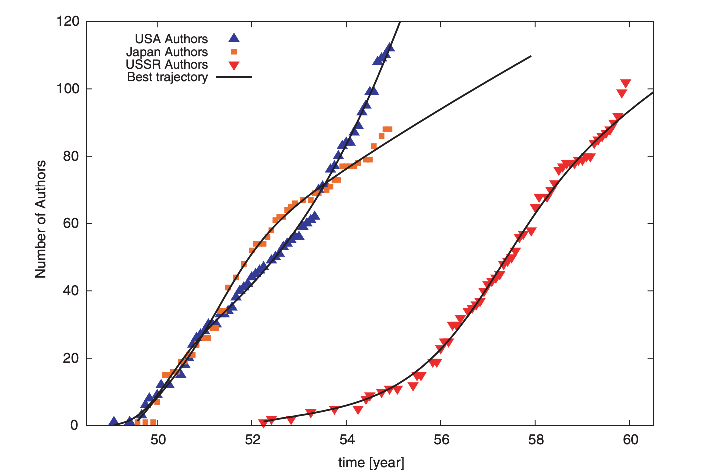
\includegraphics [width=\textwidth ]{./figures/Feynman}} \begin {flushleft}{\footnotesize Note: \cite {bettencourt2006power}, showing their fitted SEIZ model to the diffusion dynamics of Feynman diagrams in theoretical physics communities} \end {flushleft} \end {figure} \end {verbatimwrite} 

Internet memes are a favorite topic of non-economist modelers. \href{https://github.com/iworld1991/EpiExp/blob/master/Literature/bauckhage2011insights.pdf}{\cite{bauckhage2011insights}} shows that epidemiological models do a good job capturing the growth and decay of some famous memes.\ifthenelse{\boolean{inBook}}{}{ (See Figure \ref{fig:memes_curve}.)} \cite{wang2011epidemiological} finds that a modified SIR model allowing for the reinfection of the ``recovered'' fits  the propagation dynamics of various viral memes well.   A large literature has followed their work. %\href{https://github.com/iworld1991/EpiExp/blob/master/Literature/kucharski2016modelling.pdf}{\cite{kucharski2016modelling}} fits an epidemiological model to outbreaks of notable internet contagions such as the ``ice bucket challenge'' and ``no-makeup selfies.''% suggesting an initial reproduction ratio in the range of 1.9 to 2.5.

%	\href{http://cs.stanford.edu/~ashton/pubs/twiral.pdf}{\cite{goel2016structural}} explores the structural factors (independent from the intrinsic properties of the content, nature of contact process, etc.) that seem to determine whether a news story spreads more effectively from a ``broadcast'' (common-source) or from a `viral' (person-to-person) mechanism.


% Internet memes are increasingly used to sway and manipulate public opinion. This prompts the need to study their propagation, evolution, and influence across the Web. In this paper, we detect and measure the propagation of memes across multiple Web communities, using a processing pipeline based on perceptual hashing and clustering techniques, and a dataset of 160M images from 2.6B posts gathered from Twitter, Reddit, 4chan's Politically Incorrect board (/pol/), and Gab, over the course of 13 months. We group the images posted on fringe Web communities (/pol/, Gab, and The_Donald subreddit) into clusters, annotate them using meme metadata obtained from Know Your Meme, and also map images from mainstream communities (Twitter and Reddit) to the clusters. Our analysis provides an assessment of the popularity and diversity of memes in the context of each community, showing, e.g., that racist memes are extremely common in fringe Web communities. We also find a substantial number of politics-related memes on both mainstream and fringe Web communities, supporting media reports that memes might be used to enhance or harm politicians. Finally, we use Hawkes processes to model the interplay between Web communities and quantify their reciprocal influence, finding that /pol/ substantially influences the meme ecosystem with the number of memes it produces, while \td has a higher success rate in pushing them to other communities.

% There is a methodological insight for economists in these studies: To the extent that certain classes or configurations of epidemiological models are found consistently to characterize the spread of non-economic ideas (even non-textual content like videos and images), economists might be well advised to select the models that generically perform well across many kinds of content.


% \begin{center}[Insert Figure \ref{fig:memes_curve} here]\end{center}

\begin{verbatimwrite}{./Slides/FigureMemesCurve}
\begin{figure}[!ht]
  \caption{ ~Virality of internet memes: \href{https://github.com/iworld1991/EpiExp/blob/master/Literature/bauckhage2011insights.pdf}{\cite{bauckhage2011insights}}}
  \label{fig:memes_curve}
    \subfloat[``salad fingers'']{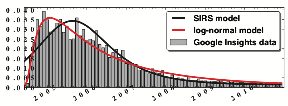
\includegraphics[width=\textwidth]{./figures/Memes1}}
    \newline
    \subfloat[``laughing baby'']{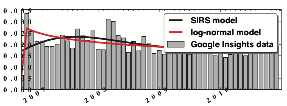
\includegraphics[width=\textwidth]{./figures/Memes2}}
    \newline
    \subfloat[``so much win'']{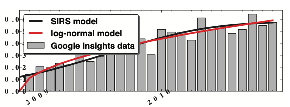
\includegraphics[width=\textwidth]{./figures/Memes3}}
    \begin{flushleft}{\footnotesize Note: This graph reproduces the SIRS model fit and log-normal fits to Google insights time series measuring the interest in six viral memes, as shown in  \cite{bauckhage2011insights}. }
    \end{flushleft}
\end{figure}

